\section {Assignment 4 \\ {Salt and Pepper Noise}}
\label {sec:assignment_4}

\subsection{Manipulate own image from assignment 2}

We applyed a salt and pepper noise filter to the image from assignment 2. The image is shown in figure \ref{fig:fortGT_Noise}.

\begin{figure}[h!]
    \centering
    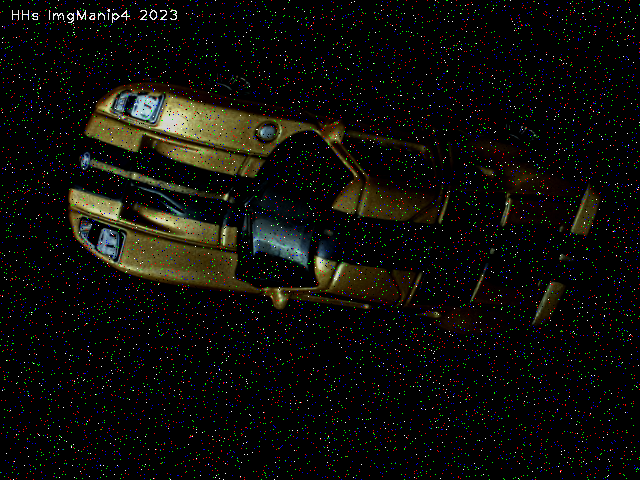
\includegraphics[width=0.45\textwidth]{fortGT_Noise.png}
    \caption{Image with salt and pepper noise}
    \label{fig:fortGT_Noise}
\end{figure}

\subsection{Write C/C++ code for Brightness correction}

\subsection{Write C/C++ code for ‘Salt and Pepper Noise’ correction}

A ‘Salt and Pepper Noise’ correction filter was written and can be found in appendix \ref{sec:appendix_B}. The filter function is shown in listing \ref{lst:noise_filter}.

\begin{lstlisting}[language=C, caption=Noise correction filter, label=lst:noise_filter]
    void filter(Mat input, Mat& result) {
        Size s = input.size();
        long h, w;
        long sum;
        
        std::cout << "Input type was : " << input.type() << std::endl;
        uint8_t out[s.height][s.width];
        
        std::cout << s.height << " " << s.width << std::endl;
        
        for (w=0; w<s.width; w++){
            for(h=0; h<s.height; h++){
                sum = 0;
                std::vector<uint8_t> median;
                
                for (int _x = -1; _x < 2; ++_x)
                {
                    for (int _y = -1; _y < 2; ++_y)
                    {
                        int idx_y = h + _y;
                        int idx_x = w + _x;
                        
                        if (idx_x < 0 || idx_x > s.width)
                            break;
                            
                        if (idx_y < 0 || idx_y > s.height)
                            break;
                        
                        median.push_back(input.at<uint8_t>(idx_y,idx_x));
                    }
                }
                std::sort(std::begin(median), std::end(median));
                        
                for (auto it = median.begin(); it != median.end(); ++it) {
                    sum = median.at(median.size()/2);
                }
                out[h][w]=(uint8_t)sum;
            }
        }
        result = Mat(s.height, s.width, CV_8U, out); //or maybe CV_8UC1?
        Size _s = result.size();
        std::cout << "done: " << _s.height << " " << _s.width << std::endl;
    }
    }
\end{lstlisting}


The result of output image is shown in figure \ref{fig:fortGT_Noise_Filtered}.

\begin{figure}[h!]
    \centering
    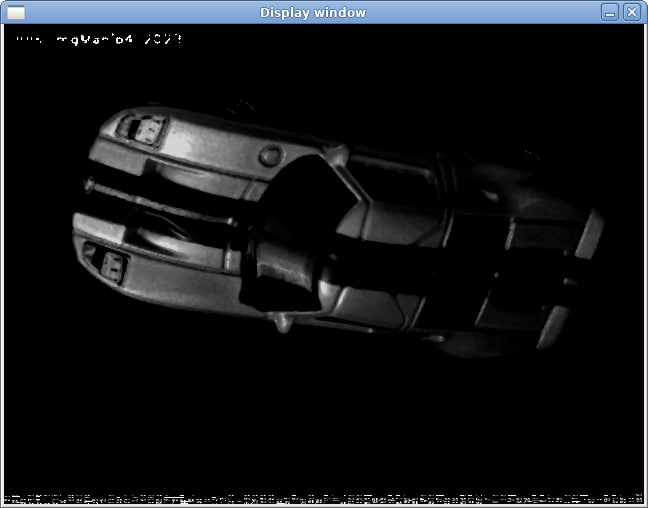
\includegraphics[width=0.45\textwidth]{fortGT_Noise_Filtered.jpg}
    \caption{Filtered image}
    \label{fig:fortGT_Noise_Filtered}
\end{figure}